\documentclass[14pt,a4paper]{extarticle}
\usepackage[T1]{fontenc}
\usepackage[utf8]{inputenc}
\usepackage[scaled]{helvet}
\renewcommand{\familydefault}{\sfdefault}
\usepackage{amsmath}
\usepackage{sansmath}
\sansmath
\usepackage[a4paper,margin=2cm]{geometry}
\usepackage{tikz}
\usetikzlibrary{angles,quotes,patterns}
\usepackage{array}
\pagestyle{empty}
% Zweite Seite: 5-mm-Kästchen, 1 cm Rand
\newcommand{\kaestchen}{\newpage\null\begin{tikzpicture}[remember picture,overlay]
\begin{scope}[shift={(current page.south west)}]\draw[step=5mm, black!45, line width=0.3pt] (1cm,1cm) grid (20cm,28.5cm);\draw[black!45, line width=0.3pt] (1cm,1cm) rectangle (20cm,28.5cm);\end{scope}
\end{tikzpicture}}
\setlength{\parindent}{0pt}
\hyphenpenalty=10000

% Nur Schwarz und Grau, die Blätter werden schwarz-weiß kopiert.
% Merkblock: Begriff und Text links, Zeichnung rechts.
\newcommand{\bl}{0.5}
\newcommand{\block}[3]{%
\begin{minipage}[c]{\bl\textwidth}\raggedright{\Large\bfseries #1\par}\medskip #2\end{minipage}\hfill
\begin{minipage}[c]{\dimexpr0.97\textwidth-\bl\textwidth\relax}\centering #3\end{minipage}\par}

\renewcommand{\bl}{0.48}
\newcommand{\basis}{\draw[thick] (0,0) -- (6,0); \fill (0,0) circle (2.5pt) node[below left] {$A$}; \fill (6,0) circle (2.5pt) node[below right] {$B$}; \node[below] at (3,0) {$c$};}
\begin{document}

{\LARGE\bfseries Dreiecke konstruieren\par}
\medskip
Ein Dreieck ist eindeutig festgelegt durch:
\vspace{0.6cm}

\block{SSS: drei Seiten}{%
Beispiel: $c = 6$\,cm, $b = 4$\,cm, $a = 5$\,cm\par\smallskip
\begin{tabular}{@{}l@{\ }>{\raggedright\arraybackslash}p{0.88\linewidth}@{}}
1. & Seite $c$ zeichnen\\
2. & Kreis um $A$ mit Radius $b$\\
3. & Kreis um $B$ mit Radius $a$\\
4. & Der Schnittpunkt ist $C$
\end{tabular}}{%
\begin{tikzpicture}[scale=1.15]
  \draw[gray, thick, dashed] (42:4) arc (42:70:4);
  \draw[gray, thick, dashed] ([shift={(6,0)}]125:5) arc (125:152:5);
  \draw[thick] (0,0) -- (2.25,3.307) -- (6,0);
  \basis
  \fill (2.25,3.307) circle (2.5pt) node[above] {$C$};
  \node[left] at (1.1,1.8) {$b$}; \node[right] at (4.2,1.8) {$a$};
\end{tikzpicture}}

\vspace{1cm}

\block{SWS: zwei Seiten und der Winkel dazwischen}{%
Beispiel: $c = 6$\,cm, $\alpha = 50^\circ$, $b = 4$\,cm\par\smallskip
\begin{tabular}{@{}l@{\ }>{\raggedright\arraybackslash}p{0.88\linewidth}@{}}
1. & Seite $c$ zeichnen\\
2. & Winkel $\alpha$ in $A$ antragen\\
3. & Auf dem Schenkel $b$ abtragen: das ist $C$\\
4. & $C$ mit $B$ verbinden
\end{tabular}}{%
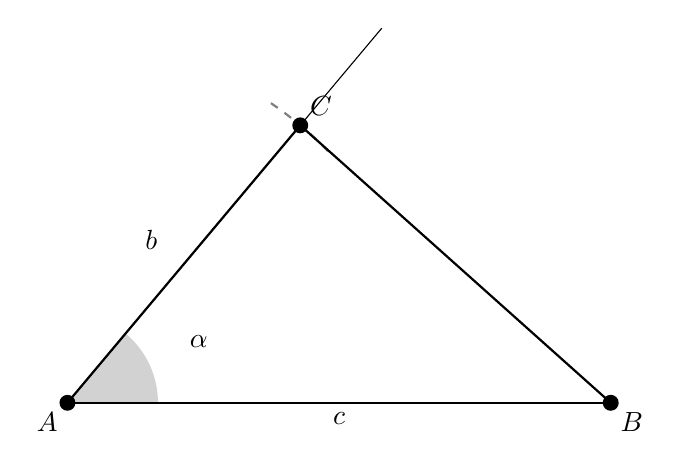
\begin{tikzpicture}[scale=1.15]
  \fill[gray!35] (0,0) -- (1,0) arc (0:50:1) -- cycle; \node at (25:1.6) {$\alpha$};
  \draw[thin] (0,0) -- (50:5.4);
  \draw[gray, thick, dashed] (44:4) arc (44:56:4);
  \draw[thick] (0,0) -- (2.571,3.064) -- (6,0);
  \basis
  \fill (2.571,3.064) circle (2.5pt) node[above right] {$C$};
  \node[left] at (1.1,1.8) {$b$};
\end{tikzpicture}}

\vspace{1cm}

\block{WSW: eine Seite und die beiden Winkel daran}{%
Beispiel: $c = 6$\,cm, $\alpha = 50^\circ$, $\beta = 60^\circ$\par\smallskip
\begin{tabular}{@{}l@{\ }>{\raggedright\arraybackslash}p{0.88\linewidth}@{}}
1. & Seite $c$ zeichnen\\
2. & Winkel $\alpha$ in $A$ antragen\\
3. & Winkel $\beta$ in $B$ antragen\\
4. & Die Schenkel schneiden sich in $C$
\end{tabular}}{%
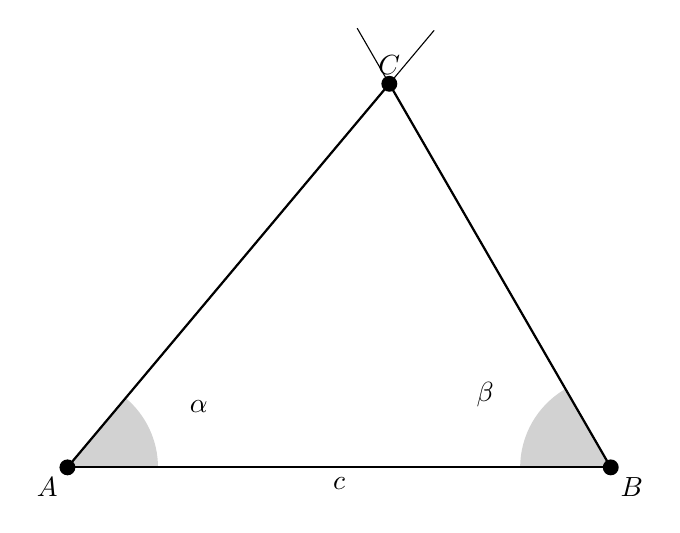
\begin{tikzpicture}[scale=1.15]
  \fill[gray!35] (0,0) -- (1,0) arc (0:50:1) -- cycle; \node at (25:1.6) {$\alpha$};
  \fill[gray!35] (6,0) -- ++(180:1) arc (180:120:1) -- cycle; \node at ([shift={(6,0)}]150:1.6) {$\beta$};
  \draw[thin] (0,0) -- (50:6.3); \draw[thin] (6,0) -- ++(120:5.6);
  \draw[thick] (0,0) -- (3.555,4.236) -- (6,0);
  \basis
  \fill (3.555,4.236) circle (2.5pt) node[above] {$C$};
\end{tikzpicture}}

\vspace{1cm}

{\Large\bfseries Aufgaben im Heft\par}
\medskip
Buch S.\,\rule{1.5cm}{0.4pt} Nr.\,\rule{5cm}{0.4pt}

\kaestchen
\end{document}
